\section{Discussion and Directions for Future Work} \label{discussion}

We have introduced motors, studied motorized games on trees, and shown that
motor-like behavior can be constructed in ordinary games, provided that each
motor has a possible firing sequence. We then showed that periodic firing
patterns are possible iff they are nonclumpy, which, among other things, allows
classification of periodic games as ``mostly waiting'' or ``mostly firing'' and
the removal of tree-like subgraphs without loss of generality.

We might expect that the space of motorized games be larger than that of
ordinary games. Theorem~\ref{natMotors} shows us that, as long as the firing
sequences involved are possible, the parallel chip-firing game is in some sense
just as ``expressive'' as its motorized variant. This allows, for example, the
simulation of some aspects of the \emph{dollar game}, a variant of the general
chip-firing game discussed by Biggs~\cite{biggs}. In the dollar game, exactly
one vertex, the ``government'', may have a negative number of chips and fires
iff no other vertices can fire. We can construct a motorized parallel
chip-firing game in which we replace the government with a motor that waits a
sufficiently large number of steps between each firing such that it never fires
in the same step as another vertex. Biggs showed that every dollar game tends
towards a critical position regardless of the order of vertex firings, so this
motorized parallel chip-firing game tends towards the same critical
position. Theorem~\ref{natMotors} may help reveal the extent to which the
parallel chip-firing game can simulate additional aspects of the dollar game
and other general chip-firing games.

% begin comment
\begin{comment}
\begin{centering}
  \begin{figure}[tbh]
    \subfloat{\includegraphics[width=\figWidthA]{Figures/motorizedTree}}
    \subfloat{\includegraphics[width=\figWidthB]{Figures/key}}
    \caption{A motor triggers a branching wave of gliders, one of which is
      shown.}
    \label{motorizedTree}
  \end{figure}
\end{centering}
\end{comment}
% end comment

Despite the expressiveness we get due to motors, the nonclumpiness of firing
patterns tells us that the parallel chip-firing game is ``easier'' than its
rules explicitly tell us it must be. In addition to results mentioned in
Section~\ref{corollaries}, Theorem~\ref{nct} is a step towards reducing the
parallel chip-firing game to one of interacting ``gliders''. For example,
consider the situation in Corollary~\ref{freeLunch}. Intuitively, we can think
of this corollary as stating that each firing of the motor creates a wave of
gliders that travels away from the motor. Every game with period at least 3 on
a cycle can be described by gliders~\cite{cycle}. (See Figure~\ref{cycleFig}.)
We believe that this approach could be used to analyze periodic behavior of
games on further classes of graphs, such as those in which each vertex is in at
most once cycle.

\begin{centering}
  \begin{figure}[tbh]
    \subfloat{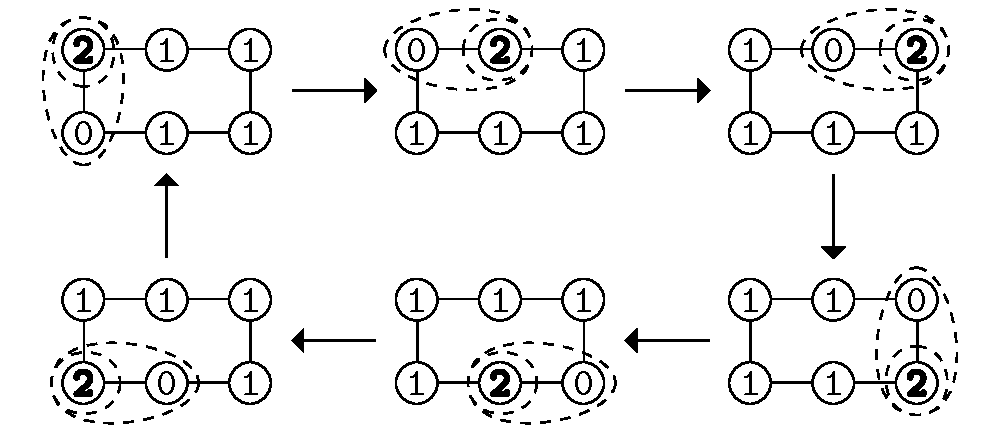
\includegraphics[width=\figWidthA]{Figures/cycle}}
    \subfloat{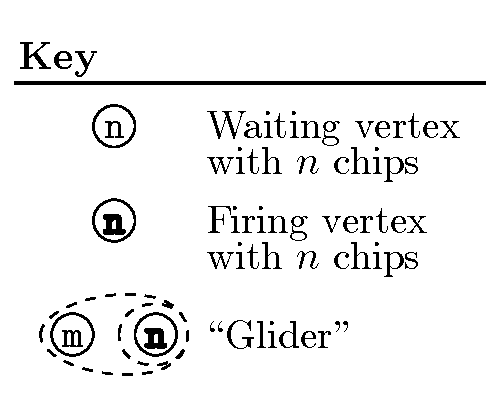
\includegraphics[width=\figWidthB]{Figures/keyShorter}}
    \caption{A game on a 6-cycle in which a glider orbits once each period.}
    \label{cycleFig}
  \end{figure}
\end{centering}

Nonclumpiness is essentially an unwritten rule of periods in the parallel
chip-firing game, which is unusual because no local property of the firing
mechanic disallows clumpiness. There are other graph automata, such as
\emph{source reversal}~\cite{sourceReversal} (essentially a parallel
chip-firing game with exactly one chip bound to each edge), that are more
restrictive than the parallel chip-firing game. For instance, nonclumpiness is
obvious for source reversal, even locally. In the other direction, motors make
it simple to show that certain stronger restrictions do not apply to the
parallel chip-firing game. For example, a path with the leaves are motors can
yield a game in which some chips cannot be bound to a single edge, which is is
a property of source reversal. We might ask which restrictions apply to which
chip-firing-style games. Is the parallel chip-firing game on undirected graphs
the most general game to which an analogue of Theorem~\ref{nct} applies?

We hope that the intuition and constructive powers of motors and the reduction
in the space of possible periodic games provided by nonclumpiness prove useful
in further research. \FloatBarrier
